%% start of file `template.tex'.
%% Copyright 2006-2013 Xavier Danaux (xdanaux@gmail.com).
%
% This work may be distributed and/or modified under the
% conditions of the LaTeX Project Public License version 1.3c,
% available at http://www.latex-project.org/lppl/.

\documentclass[11pt,a4paper,sans]{moderncv}        % possible options include font size ('10pt', '11pt' and '12pt'), paper size ('a4paper', 'letterpaper', 'a5paper', 'legalpaper', 'executivepaper' and 'landscape') and font family ('sans' and 'roman')

\usepackage[percent]{overpic}
\usepackage{tikz}
\usepackage{fontawesome5}

% moderncv themes
\moderncvstyle{classic}                             % style options are 'casual' (default), 'classic', 'oldstyle' and 'banking'
\moderncvcolor{my}                               % color options 'blue' (default), 'orange', 'green', 'red', 'purple', 'grey' and 'black'
%\renewcommand{\familydefault}{\sfdefault}         % to set the default font; use '\sfdefault' for the default sans serif font, '\rmdefault' for the default roman one, or any tex font name
%\nopagenumbers{}                                  % uncomment to suppress automatic page numbering for CVs longer than one page

% character encoding
\usepackage[utf8]{inputenc}                       % if you are not using xelatex ou lualatex, replace by the encoding you are using
%\usepackage{CJKutf8}                              % if you need to use CJK to typeset your resume in Chinese, Japanese or Korean

% adjust the page margins
\usepackage[scale=0.75]{geometry}
%\setlength{\hintscolumnwidth}{3cm}                % if you want to change the width of the column with the dates
%\setlength{\makecvtitlenamewidth}{10cm}           % for the 'classic' style, if you want to force the width allocated to your name and avoid line breaks. be careful though, the length is normally calculated to avoid any overlap with your personal info; use this at your own typographical risks...
\newcommand{\iconHref}{\raise.2ex\hbox{{\tiny\faLink}}\hspace{0.2em}}

% personal data
\name{Dominik}{Gmiterko}
\title{Coder | Artist | Me}                               % optional, remove / comment the line if not wanted
%\address{street and number}{postcode city}{country}% optional, remove / comment the line if not wanted; the "postcode city" and and "country" arguments can be omitted or provided empty
\email{d.gmiterko@gmail.com}                               % optional, remove / comment the line if not wanted
\homepage{deegmiterko.com}                         % optional, remove / comment the line if not wanted
\phone[mobile]{+420~703~996~858}                   % optional, remove / comment the line if not wanted
%\phone[fixed]{+2~(345)~678~901}                    % optional, remove / comment the line if not wanted
%\phone[fax]{+3~(456)~789~012}                      % optional, remove / comment the line if not wanted
%\extrainfo{additional information}                 % optional, remove / comment the line if not wanted
\social[linkedin]{dominik-gmiterko}
\social[github]{dee-gmiterko}
\photo[100pt][0.2pt]{img/picture}                       % optional, remove / comment the line if not wanted; '64pt' is the height the picture must be resized to, 0.4pt is the thickness of the frame around it (put it to 0pt for no frame) and 'picture' is the name of the picture file
% \quote{Some quote}                                 % optional, remove / comment the line if not wanted

% to show numerical labels in the bibliography (default is to show no labels); only useful if you make citations in your resume
%\makeatletter
%\renewcommand*{\bibliographyitemlabel}{\@biblabel{\arabic{enumiv}}}
%\makeatother
%\renewcommand*{\bibliographyitemlabel}{[\arabic{enumiv}]}% CONSIDER REPLACING THE ABOVE BY THIS

% bibliography with mutiple entries
%\usepackage{multibib}
%\newcites{book,misc}{{Books},{Others}}
%----------------------------------------------------------------------------------
%            content
%----------------------------------------------------------------------------------
\begin{document}
%\begin{CJK*}{UTF8}{gbsn}                          % to typeset your resume in Chinese using CJK
%-----       resume       ---------------------------------------------------------
\makecvtitle


\section{Experience}
\cventry{2022--2024}{Product developer}{Freelance}{}{}{Directly assisting clients with tailored full-stack solutions "from analysis to analytics"}
\cventry{2019--2022}{Data Engineer}{Kiwi.com}{Brno}{}{Building and maintaining data pipelines, contributing to the formation of a data warehouse, and assisting with analysis and visualization, while ensuring data quality}
\cventry{2017--2019}{Web Frontend}{InQool a.s.}{Brno}{}{Creating custom web applications for e-shops. Notably, I've worked on \href{https://www.brnoid.cz/}{\iconHref{}Brno iD}}
\cventry{2015--2016}{Web Backend}{WAME.sk}{Bardejov}{}{Developer of custom e-commerce solutions in a small team}


\section{Education}
\cventry{2018--2020}{Artificial Intelligence and Data Processing*}{Master's degree}{Faculty of Informatics, Masaryk University}{}{*Not formally finalized}
\cventry{2015--2018}{Computer Systems and Data Processing}{Bachelor's degree}{Faculty of Informatics, Masaryk University}{}{}
\cvitem{2010--2015}{\textit{Technické lýceum}, Stredná priemyselná škola, Bardejov}


\section{Masters thesis}
\cvitem{Title}{\emph{Tool Supporting Analysis of Meteorology Data}}
\cvitem{Supervisor}{RNDr. Tomáš Rebok, Ph.D.}
\cvitem{}{A newly built system allowing users to process and validate meteorological data while enhancing the analytical capabilities.}
\cvitem{Url}{\href{https://is.muni.cz/th/vaev3/tool-supporting-analysis-of-meteorology-data.pdf}{\iconHref{}Full text}}

\clearpage

\section{Bachelors thesis}
\cvitem{Title}{\emph{Techniques for measuring similarity of educational items}}
\cvitem{Supervisor}{doc. Mgr. Radek Pelánek, Ph.D.}
\cvitem{}{Using machine learning to measure the similarity of questions in tutoring systems utilizing only the correctness of answers from users.}
\cvitem{Url}{\href{https://is.muni.cz/th/l5dzj/gmiterko-similarity.pdf}{\iconHref{}Full text}, excerpt: \href{http://ienze.me/tmsei\_thesis/}{\iconHref{}ienze.me/tmsei\_thesis}}


% banner
\begin{center}
\href{http://deegmiterko.com}{
  \begin{overpic}[width=\textwidth]{img/banner}
   \put (15,7) {\LARGE\mdseries\slshape\color{white}http://deegmiterko.com}
   \put (15,3) {\large\slshape\color{white}50+ small personal projects}
  \end{overpic}
}
\end{center}


\section{Skills}
\begin{cvcolumns}
  \cvcolumn{User-facing}{\begin{itemize}
    \item Javascript, Typescript,
    \item React, WebGL, Unity,
    \item CSS and preprocessors,
    \item UI/UX design.
  \end{itemize}}
  \cvcolumn{Business logic}{\begin{itemize}
    \item Python, Java,
    \item SQL databases,
    \item Document stores,
    \item C++, Testing.
  \end{itemize}}
  \cvcolumn{Operations}{\begin{itemize}
    \item Airflow, Jupyter, DBT,
    \item AI, Machine learning,
    \item Google Cloud, Docker,
    \item Linux, Kubernetes.
  \end{itemize}}
\end{cvcolumns}
\cvitemwithcomment{\textit{Languages}}{English \textit{(Fluent)}, Slovak \textit{(Native)}, Czech}{}

% \section{Languages}
% \cvitemwithcomment{English}{Fluent}{}
% \cvitemwithcomment{Slovak}{Native}{}



% \section{Interests}
% \cvitem{Organizing}{Organizing of competitions, primarily online logic team competition InterLoS}
% \cvitem{Travel}{I enjoy discovering new hidden places}
% \cvitem{Drawing}{\includegraphics[height=10pt]{1f58d}}


\section{Last notable project}
\cventry{2024}{Na medicínu}{Internal system for a study course}{\href{https://namedicinu.cz}{\iconHref{}namedicinu.cz}}{}{}{}
\cvitem{}{\textit{An application where students can find all necessary materials in one place, practice, and watch lectures. While giving lecturers quantitative data about what topics need to be covered better.}}
\cvlistdoubleitem{Lecture recordings,}{Video encoding and streaming,}
\cvlistdoubleitem{Flashcard training,}{Generating quizzes for testing,}
\cvlistdoubleitem{User analytics,}{Lecturer insights about students.}

% \section{References}
% \begin{cvcolumns}
%  \cvcolumn{Category 1}{\begin{itemize}\item Person 1\item Person 2\item Person 3\end{itemize}}
%  \cvcolumn{Category 2}{Amongst others:\begin{itemize}\item Person 1, and\item Person 2\end{itemize}(more upon request)}
%  \cvcolumn[0.5]{All the rest \& some more}{\textit{That} person, and \textbf{those} also (all available upon request).}
% \end{cvcolumns}

% Publications from a BibTeX file without multibib
%  for numerical labels: \renewcommand{\bibliographyitemlabel}{\@biblabel{\arabic{enumiv}}}% CONSIDER MERGING WITH PREAMBLE PART
%  to redefine the heading string ("Publications"): \renewcommand{\refname}{Articles}
\nocite{*}
\bibliographystyle{plain}
\bibliography{publications}                        % 'publications' is the name of a BibTeX file

% Publications from a BibTeX file using the multibib package
%\section{Publications}
%\nocitebook{book1,book2}
%\bibliographystylebook{plain}
%\bibliographybook{publications}                   % 'publications' is the name of a BibTeX file
%\nocitemisc{misc1,misc2,misc3}
%\bibliographystylemisc{plain}
%\bibliographymisc{publications}                   % 'publications' is the name of a BibTeX files

\begin{tikzpicture}[remember picture,overlay,shift={(current page.north east)}]
\node[anchor=north east,xshift=4pt,yshift=-650pt]{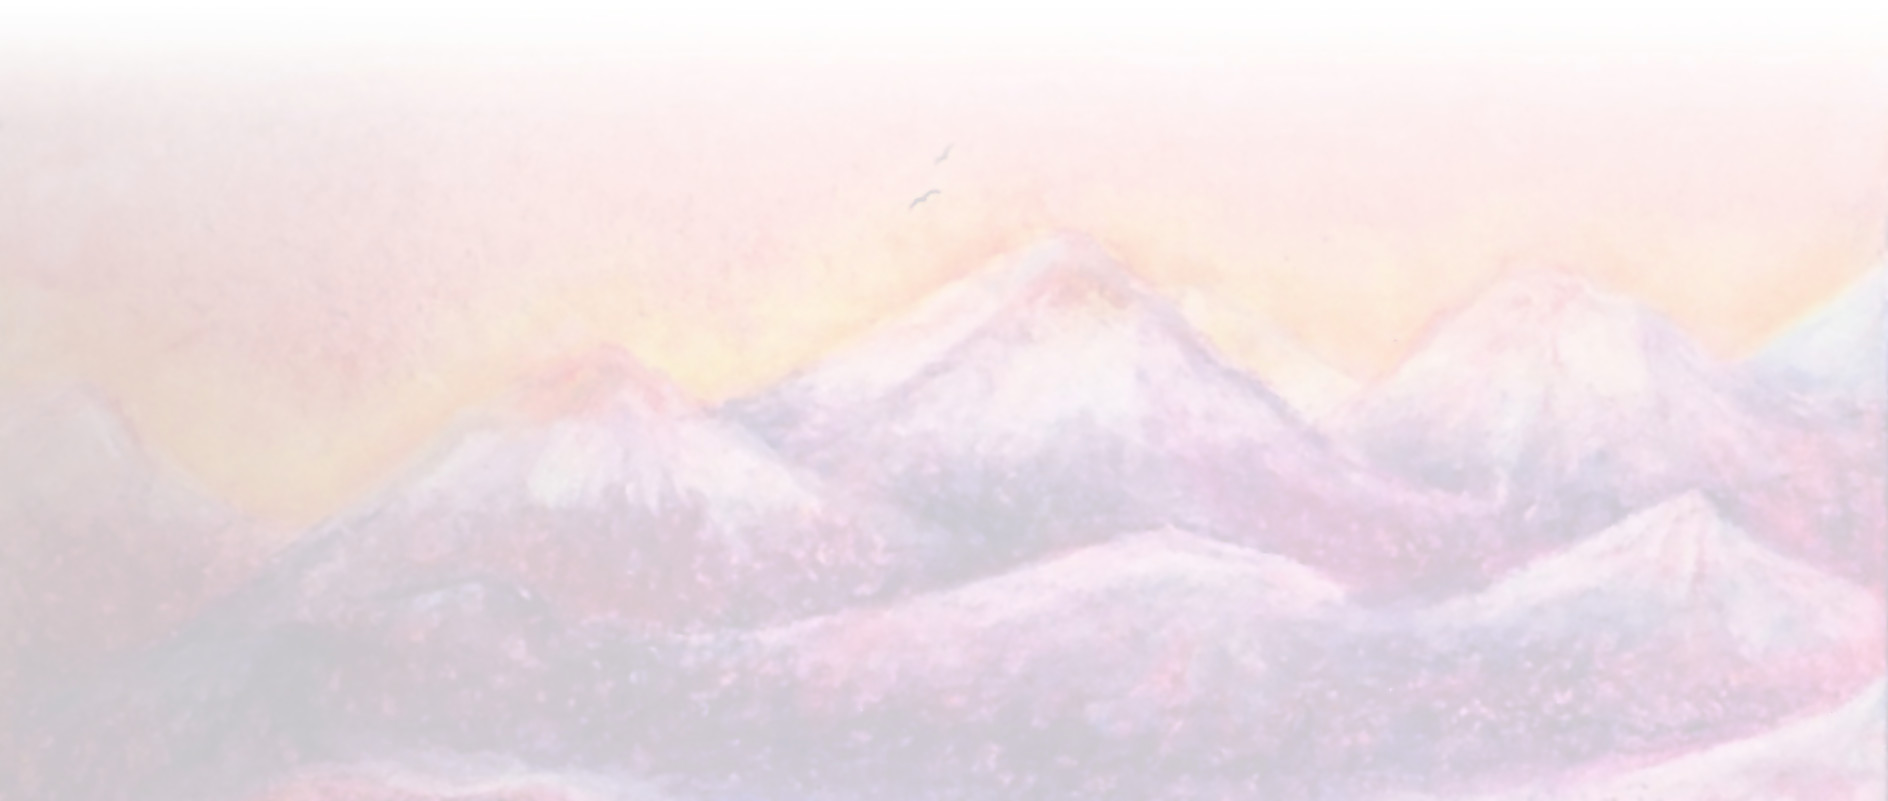
\includegraphics[width=\paperwidth]{img/cv_bg}};
\end{tikzpicture}

\clearpage
%-----       letter       ---------------------------------------------------------
% recipient data
%\recipient{Company Recruitment team}{Company, Inc.\\123 somestreet\\some city}
%\date{January 01, 1984}
%\opening{Dear Sir or Madam,}
%\closing{Yours faithfully,}
%\enclosure[Attached]{curriculum vit\ae{}}          % use an optional argument to use a string other than "Enclosure", or redefine \enclname
%\makelettertitle
%
%Lorem ipsum dolor sit amet, consectetur adipiscing elit. Duis ullamcorper neque sit amet lectus facilisis sed luctus nisl iaculis. Vivamus at neque arcu, sed tempor quam. Curabitur pharetra tincidunt tincidunt. Morbi volutpat feugiat mauris, quis tempor neque vehicula volutpat. Duis tristique justo vel massa fermentum accumsan. Mauris ante elit, feugiat vestibulum tempor eget, eleifend ac ipsum. Donec scelerisque lobortis ipsum eu vestibulum. Pellentesque vel massa at felis accumsan rhoncus.
%
%Suspendisse commodo, massa eu congue tincidunt, elit mauris pellentesque orci, cursus tempor odio nisl euismod augue. Aliquam adipiscing nibh ut odio sodales et pulvinar tortor laoreet. Mauris a accumsan ligula. Class aptent taciti sociosqu ad litora torquent per conubia nostra, per inceptos himenaeos. Suspendisse vulputate sem vehicula ipsum varius nec tempus dui dapibus. Phasellus et est urna, ut auctor erat. Sed tincidunt odio id odio aliquam mattis. Donec sapien nulla, feugiat eget adipiscing sit amet, lacinia ut dolor. Phasellus tincidunt, leo a fringilla consectetur, felis diam aliquam urna, vitae aliquet lectus orci nec velit. Vivamus dapibus varius blandit.
%
%Duis sit amet magna ante, at sodales diam. Aenean consectetur porta risus et sagittis. Ut interdum, enim varius pellentesque tincidunt, magna libero sodales tortor, ut fermentum nunc metus a ante. Vivamus odio leo, tincidunt eu luctus ut, sollicitudin sit amet metus. Nunc sed orci lectus. Ut sodales magna sed velit volutpat sit amet pulvinar diam venenatis.
%
%Albert Einstein discovered that $e=mc^2$ in 1905.
%
%\[ e=\lim_{n \to \infty} \left(1+\frac{1}{n}\right)^n \]
%
%\makeletterclosing

%\clearpage\end{CJK*}                              % if you are typesetting your resume in Chinese using CJK; the \clearpage is required for fancyhdr to work correctly with CJK, though it kills the page numbering by making \lastpage undefined
\end{document}


%% end of file `template.tex'.
